\subsection{Detector Support System}
\label{sec:fdsp-tc-infr-dss}


The \dword{dss} provides the structural support for the detector inside the cryostat.  
It also provides the necessary infrastructure inside the cryostat to move the detector elements into place during assembly. 
The \dword{dss} is a new design, quite different from the \dword{pdsp} \dword{dss}. The detector elements supported by the \dword{dss} include the \dwords{ewfc}, the \dword{apa}s, and the \dwords{cpa} with top and bottom \dword{fc} panels. 
The nominal load of the detector elements both dry (in air) and wet (in \dword{lar}) are shown in Table~\ref{tab:installation-DSS-load}. 
The weights listed are the current design weights.  
The \dword{dss}, however, is designed to accommodate significant design changes --- even if the detector weight were to double the \dword{dss} would still meet the design code requirements.  
Deformations would increase due to any increase in loads, and this effect would be evaluated if needed.

\begin{dunetable}
[DSS Loads]
{l|c|cc|cc}
{tab:installation-DSS-load}
{The expected dry and wet stratic loads for the DSS. \fixme{Vic and Farshid need to vet this table.}}
%\multicolumn{2}{c}{} &  \multicolumn{4}{|c}{Dry Weight}\\ \toprowrule
& &  \multicolumn{4}{|c}%{Dry Weight}
{Weight before fill (Dry)}\\ \toprowrule
& & \multicolumn{2}{c|}{Unit Weight} & \multicolumn{2}{c|}{Total Weight}  \\ \colhline

Detector Component &\# Units& (kg)&(lbs) & (kg) &(lbs)\\ \colhline
\dword{dss} & 1 &NA&NA& 12318  & 27100 \\ 
\colhline
\dword{apa} (Installed \dword{apa} pair, no cables)& 75&1184 &2604 &88768  &195290\\ 
\colhline
\dword{cpa} & 100& 233 & 513 & 23331 & 51327 \\ 
\colhline
Top or Bottom \dword{fc} module (FC TB)& 400&149 & 328	 & 59679 & 131294\\ 
\colhline
\dword{ce} Cables &750& 182 & 400 & 13636 & 30000\\
\colhline
\dword{ewfc}  & 8	&904 &	1989  & 7234 & 15914\\ 
\colhline
{\bf Total} &  & & & 204966 &	450925\\ 
\colhline
\toprowrule

\rowtitlestyle & &  \multicolumn{4}{c}{Weight after fill (Wet)}\\
\toprowrule
\dword{dss} (not in liquid) & 1 & NA & NA & 12318 & 27100 \\ 
\colhline
\dword{apa} (Installed \dword{apa} pair/No cables)&75& &0 & 0 &0\\ 
\colhline
\dword{cpa} & 100& 45 & 99 & 4520 & 9943 \\ 
\colhline
Top or Bottom \dword{fc} module (FC TB)& 400 & 68 & 150	& 27359 & 60191 \\ 
\colhline
\dword{ce} Cables & 75 & & & 13636& 30000 \\
\colhline
\dword{ewfc}  & 8 & 283& 	622& 2263 & 4978\\  
\colhline
{\bf Total} &  & & &60096	 &132211 \\ 
\colhline
\end{dunetable}


The \dword{dss} shown in Figure~\ref{fig:DSS} consists of five rows of I-beams inside the detector that support the five rows of \dword{apa}s and \dword{cpa}s. 
The I-beams themselves are supported from the cryostat outer steel structure through a series of vertical supports or mechanical \fdth{}s, also shown in Figure~\ref{fig:DSS}. 
The \dword{dss} constrains the location of the detector inside the cryostat and also accommodates the detector elements' movement and contraction during cooling. The design of the \dword{dss} sets the overall structure of the \dword{detmodule} since only after the elements are mounted to the \dword{dss} and connected do they make a unified mechanical structure. 
During installation the detector components are moved along the I-beams using both simple and motorized trolleys. 
The end of the \dword{dss} nearest the \dword{tco} is also designed as a switchyard. An additional set of north-south beams allow a short section of the I-beam rail to be shifted between the five rows of \dword{dss} beams that correspond to the five alternating rows of detector elements  (\dword{apa}-\dword{cpa}-\dword{apa}-\dword{cpa}-\dword{apa}).  
With this the \SI{12}{m} tall detector elements can enter the cryostat on an I-beam through the \dword{tco}, be loaded on the short switchyard beam, moved to the required row of \dword{dss} and then be pushed into position. 
\fixme{add reference to TC vol Ch 7 fig 7.6}

\begin{dunefigure}[\threed model of the DSS] {fig:DSS}
  {\threed model of the \dword{dss} showing the entire
  structure on the left along with one \dword{apa} row and one
  \dword{cpa}-\dword{fc} row at each end. The right panel is a zoomed image
  showing the connections between the vertical supports and the
  horizontal I-beams.}
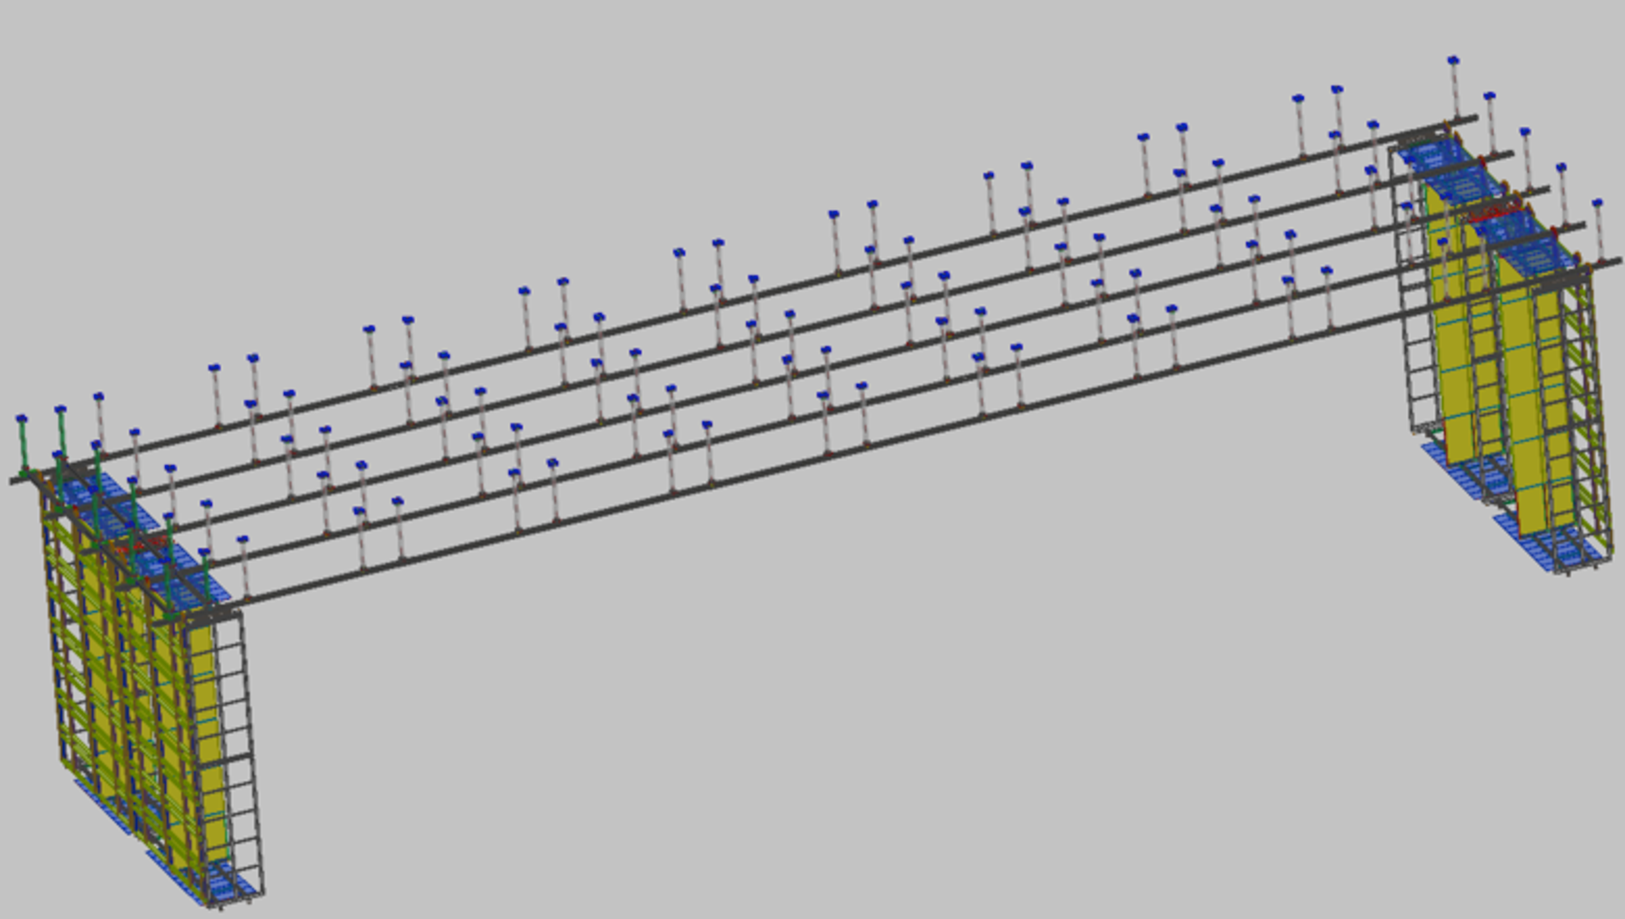
\includegraphics[width=.49\textwidth]{DSS-1.pdf}
 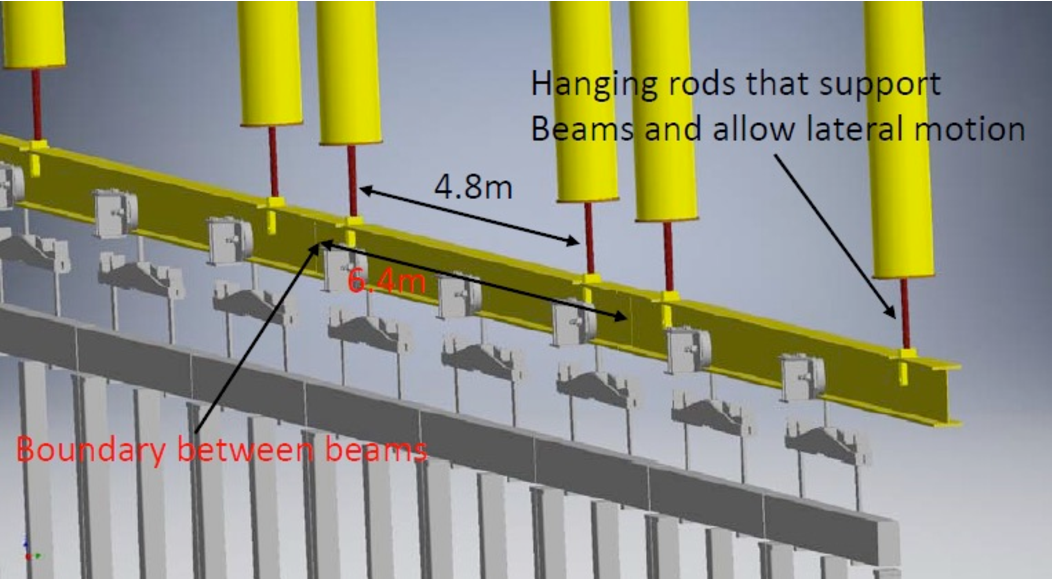
\includegraphics[width=.49\textwidth]{DSS-2.pdf}
\end{dunefigure}


% \textquotedblleft cryostat crossing tubes\textquotedblright\   that penetrate the cryostat insulation.  \ref{fig:crossingtube}


The \dword{dss} is designed to meet the following  requirements:
\fixme{nonstandard list formatting. Why? Anne}
\begin{itemize}
 \setlength\itemsep{1mm}
\setlength{\parsep}{1mm}
\setlength{\itemsep}{-5mm}
% \small
\item Support the weight of the detector;
\item Accommodate cryostat roof movement during filling, testing, and operation;
\item Accommodate variation in \fdth locations and
  variation in the flange angles due to installation tolerances and
  loading on the warm structure;
\item Accommodate shrinkage of the detector and \dword{dss} from ambient
  temperature to \dword{lar} temperature;
\item Define the positions of the detector components relative to each other; 
\item Provide electrical connection to the cryostat ground and remain electrically isolated from the detector;
\item Allow support penetrations to be purged with gaseous argon to prevent contaminants from diffusing back into the liquid; 
\item Ensure that the instrumentation cabling does not interfere with the \dword{dss};
\item Consist entirely of components that can  
be installed through the \dword{tco};
\item Meet AISC-360 codes; 
\item Meet seismic requirements one mile underground at \dword{surf};
\item Consist entirely of materials compatible %for 
with operation in ultrapure \dword{lar};
\item Ensure that the \dword{dss} beams either sit completely submerged in \dword{lar} or sit completely in gas while leaving a \SI{4}-\SI{5}{\%} ullage at the top of the cryostat;  
%\item Centerline of the \dword{apa} near the cryostat wall shall be \SI{400}{mm} from the membrane flat surface;
\item Maintain the centerline of the \dword{apa} near the cryostat at \SI{400}{mm} from the membrane flat surface;
\item Ensure that the supports do not interfere with the cryostat I-beam structures;
\item Ensure that the detector's lower \dword{gp} lies over the cryogenic piping;
%and that the tops of the \dword{dss} beams are either fully submerged in \dword{lar} or fully in gas while leaving a \SI{4}-\SI{5}{\%} ullage at the top of the cryostat; 
\item Include the infrastructure necessary to move the \dword{apa} and \dword{cpa}-\dword{fc} assemblies from outside the cryostat through the \dword{tco} to the correct position.
\end{itemize}

Each row of the \dword{dss} consists of a series of \num{10} \SI{6.4}{m} long
W10$\times$26 stainless steel I-beam sections, for a total of \num{50} I-beam segments for the five rows. The length of the beam segments was chosen to be a multiple of the \SI{1.6}{m} pitch of the major cryostat beams, which allows the regular placement of the support \fdth across the cryostat roof. With a W10$\times$26 I-beam and \SI{6.4}{m} between the supports,  the beam deflections due to the loads was \fixme{can be?} kept below \SI{5}{mm}. 
Each I-beam is suspended on both ends by the mechanical \fdth{}s that penetrate the cryostat roof. 
During \cooldown  each I-beam shrinks while the mechanical supports outside the cryostat remain fixed,  causing gaps to form between \dword{apa}s that are adjacent but supported on separate beams.
\dword{apa}s that are supported on the same beam will not have gaps develop because both the beam and \dword{apa} frames are stainless steel and will shrink together.
The gap between two adjacent \dword{dss} beams after \cooldown will be \SI{17}{mm}; this is considered acceptable. 
Increasing the the beam length beyond \SI{6.4}{m} was not considered because the deformation of the I-beam under load would increase, as would the gap between \dword{apa}s on adjacent beams and the difficulty of installing the beams. % would increase.
\fixme{need max deflection number from Vic}


\begin{dunefigure}[DSS vertical support \fdth]{fig:DSS-Support}
  { Drawing of the \dword{dss} vertical support \fdth. The detector load is carried by the \SI{25}{mm} inner support rod. The outer lateral support tube prevents swinging during installation.  The \fdth mounts to the cryostat crossing tube, which is an integral part of the cryostat. Not shown here are the short vacuum chambers for the \dword{cisc} instrumentation; these are shown in Figure \ref{fig:CISC-feedthru}.}
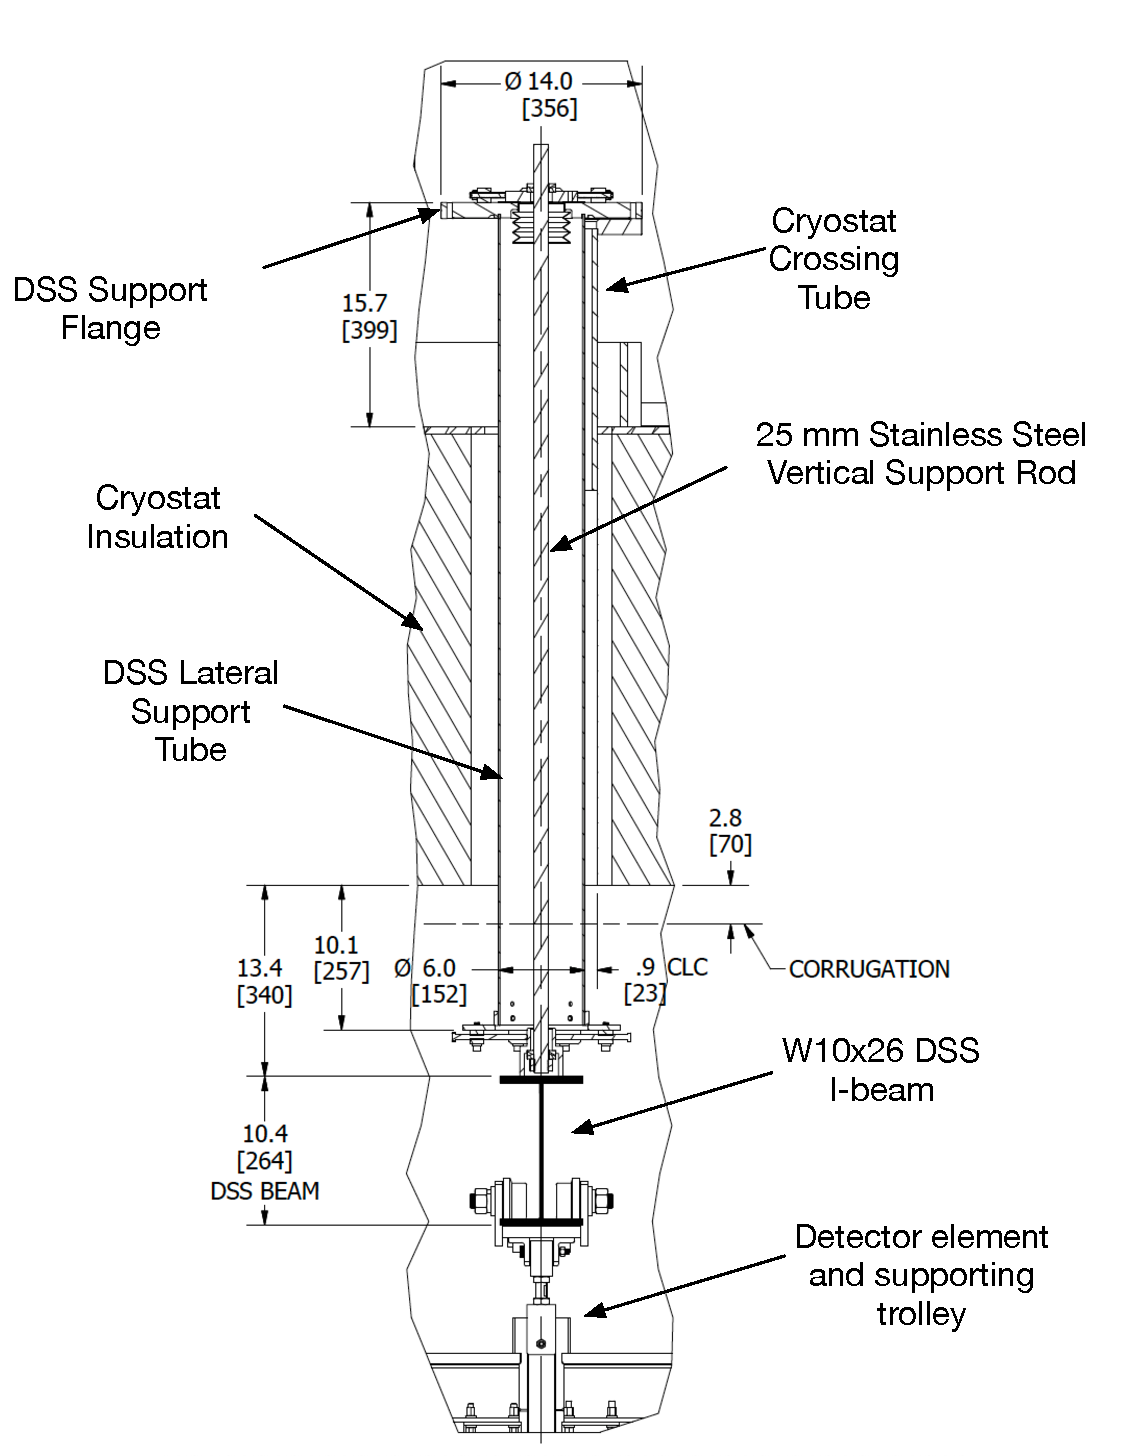
\includegraphics[width=.85\textwidth]{graphics/DSS-Support.pdf}
\end{dunefigure}


The \dword{dss} I-beams are supported on both ends from a vertical support \fdth shown in Figure~\ref{fig:DSS-Support}. A \SI{25}{mm} solid stainless steel rod, which is threaded at both ends, runs down the center of the \fdth and carries the detector load. The support rod connects on the bottom end to a clevis which is then pinned to the \dword{dss} beams shown in Figure \ref{fig:DSS-lateral-support}. At the top the rod bolts to an X-Y table sitting on the top Conflat Flange that allows a lateral adjustment of $\pm$\SI{2.5}{cm} (\SI{1}{in}). A swivel washer is used in the bolted connection to the X-Y table to allow the support rod to swing freely. The bolted connection also allows the \dword{dss} I-beams to be adjusted vertically. The vacuum seal is established at the top with a bellows between the rod and the top flange. The top flange of the \dword{dss} support \fdth is a Conflat flange that connects to the cryostat crossing tube's mating flange. The crossing  tube is welded to the cryostat roof and the top flange is mechanically supported from the cryostat's  \SI{1.1}{m} tall support I-beams. The cryostat crossing tubes are shown in Figure~\ref{fig:crossingtube}.

During installation the detector components will be pushed along the \dword{dss} I-beams, placing a lateral load on the \dword{dss}. % support structure. 
A \SI{15.2}{cm} (\SI{6}{in}) \dword{od}  tube is welded to the top flange of the \dword{dss} \fdth{}. 
This lateral support tube  extends through the cryostat insulation and has a clamping collar at the bottom that is used to fix the I-beam support clevises in position during installation. 
The bottom of the lateral support tube is seen in Figure~\ref{fig:DSS-lateral-support}. 
The long bolts press on the flat sides of the clevis to fix the support rod's location. 
There is a nominal \SI{10}{mm} gap between the \dword{od} of the support tube and the \dword{id} of the clearance tube in the cryostat. 
The clevis can be positioned anywhere inside the \SI{15.2}{cm} tube.




\begin{dunefigure}[DSS support for lateral loads ]{fig:DSS-lateral-support}
  {Left panel shows how the central support rod is locked in position during detector installation. The outer  \SI{15.2}{cm} (\SI{6}{in}) tube is used to fix the support clevis in position. The right panel shows the system as it is connected to the I-Beam.}
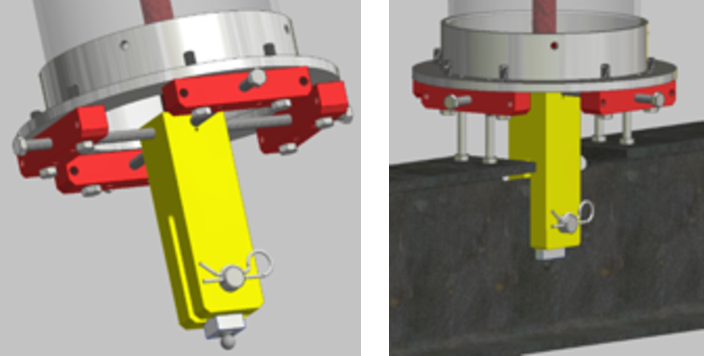
\includegraphics[width=.75\textwidth]{graphics/dss-lateral-support.pdf}
\end{dunefigure}

After the detector has been installed all restraints on the clevis are released to allow motion as the detector contracts during \cooldown.  The two support rods that support each \dword{dss} beam will contract and move toward each other by \SI{13.1}{mm} along the axis of the detector.  
The drift distance will shrink by \SI{7.4}{mm}  caused by the contraction of the field cage.  The detector is symmetric in the drift direction around the center \dword{apa}.  The drifts on either side of the center \dword{apa} will  shrink toward the center while the center \dword{apa} remains unmoved.  This results in the \dword{cpa}s moving \SI{7.4}{mm}  toward the center and the outer \dword{apa}s moving \SI{14.8}{mm}  (2$\times$\SI{7.4}{mm}) toward the center.  The hanging rod is designed to have a range of motion of \SI{15}{mm}  in the drift direction to accommodate this shrinkage.




Detector components are installed using a shuttle beam system as
illustrated in Figure~\ref{fig:shuttle}.  
The last two columns of \fdth{}s (western-most) support temporary beams that run
north-south, perpendicular to the main \dword{dss} beams.  
A shuttle beam has trolleys mounted to it and traverses 
north-south until it aligns with the required row of \dword{dss} beams.  
The last \dword{apa} or \dword{cpa} in a row is supported by the shuttle beam, which is bolted directly to the \fdth{}s once it is in place.  
As the last \dword{cpa} or \dword{apa} in each row is installed, the north-south beams are removed.

\begin{dunefigure}[\threed models of the shuttle beam end of the DSS]{fig:shuttle}
  {\threed models of the shuttle beam end of the \dword{dss}. The figures show how an \dword{apa}
is translated into position using the north-south beams until it lines up with the correct
row of I-beams.}
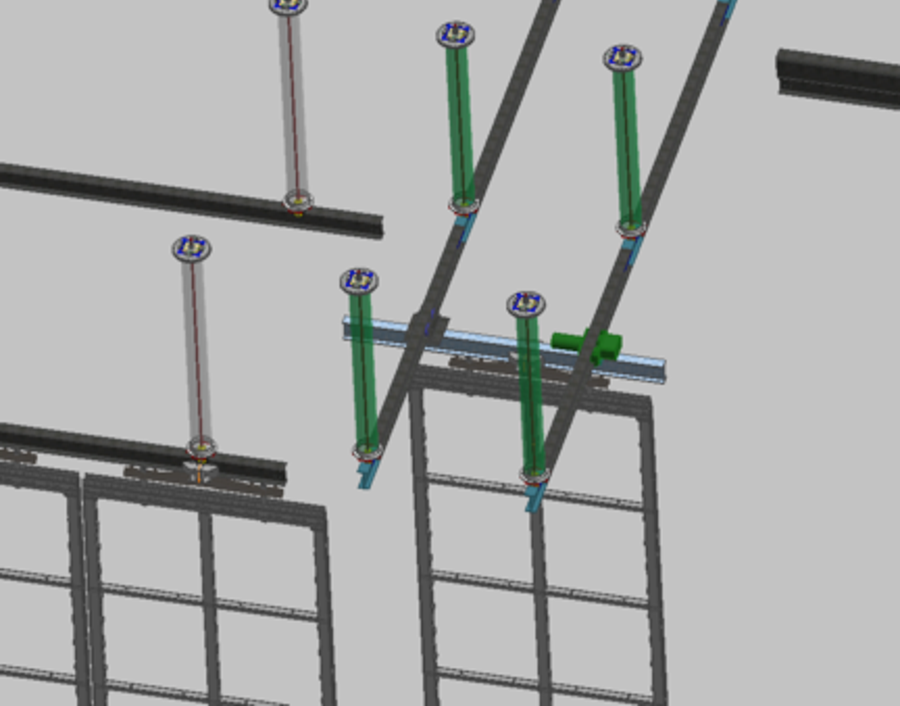
\includegraphics[width=.49\textwidth]{/Shuttle-1.pdf}
 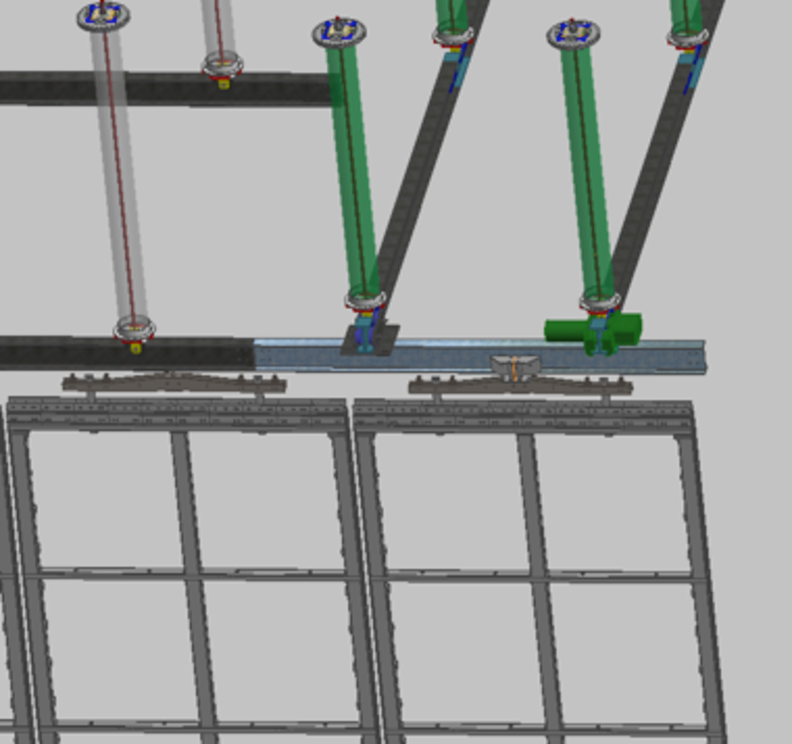
\includegraphics[width=.42\textwidth]{shuttle-2.pdf}
\end{dunefigure}

%A mechanical stop  prevents trolleys from passing the end of the shuttle beam unless it is aligned with acorresponding \dword{dss} beam.  The shuttle beam and each detector component are moved using a motorized trolley.  A commercially available motorized trolley will be modified as needed for the installation. 
The shuttle beam and each detector component are moved using a motorized trolley.  A commercially available motorized trolley will be modified as needed for the installation. A mechanical stop will prevent the trolley from passing the end of the shuttle beam unless the beam is aligned with a corresponding \dword{dss} beam. 


\begin{dunefigure}[Prototype of the motorized DSS trolley ]{fig:DSS-trolley}
  {Prototype of the motorized \dword{dss} trolley that will push the \dword{apa} and \dword{cpa} along the I-beams and through the switchyard.}
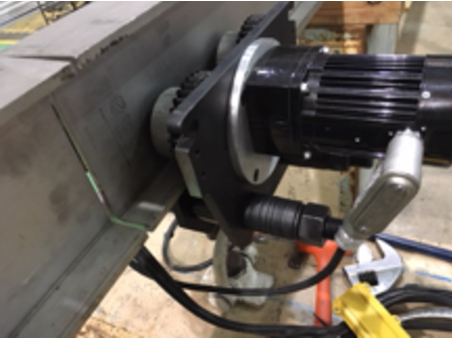
\includegraphics[width=.49\textwidth]{graphics/DSS-trolley.pdf}
\end{dunefigure}



A mock-up of the shuttle system will be constructed to test the
mechanical interlock and drive systems for the shuttle beam
for each \dword{detmodule}.  Tests will be conducted to evaluate the level of
misalignment between beams that can be tolerated and the amount of
positional control that can be achieved with the motorized trolley. We plan to construct a full scale prototype of a section of the  switchyard and perform tests at floor level. Later, the test program will be expanded at Ash River, where a full-scale installation test will be performed; see  
Section~\ref{sec:fdsp-tc-infr-qaqc}.
